\documentclass[border=4pt]{standalone}

\usepackage[T1]{fontenc}
\usepackage[utf8]{inputenc}
\usepackage{amsmath}
\usepackage{xcolor}
\usepackage{tikz}
\usetikzlibrary{positioning, calc, arrows.meta, backgrounds}

\definecolor{curvec}{RGB}{45,109,180}   % schedule curve : blue

\begin{document}

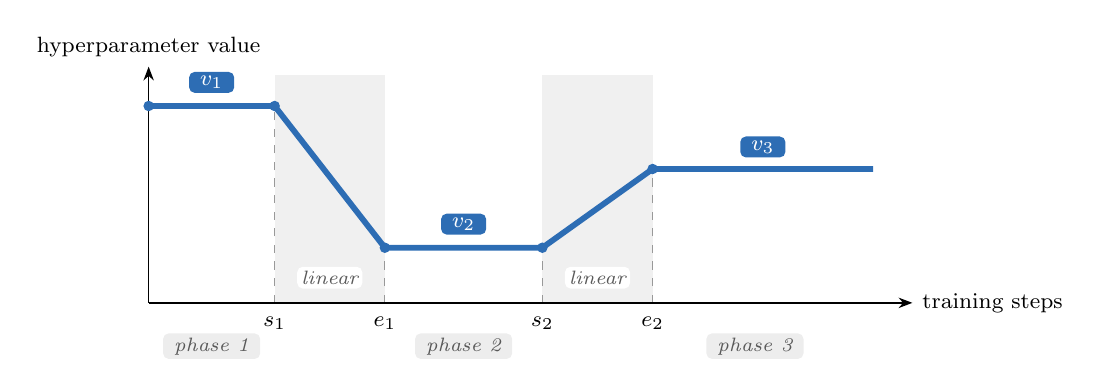
\begin{tikzpicture}[font=\small, >={Stealth[length=5pt]}]

% boundaries: s1=1.6, e1=3.0, s2=5.0, e2=6.4 ; plateaus v1=2.5, v2=0.7, v3=1.7

%% ── transition bands (background) ────────────────────────────────
\begin{scope}[on background layer]
  \fill[black!6] (1.6,0) rectangle (3.0,2.9);
  \fill[black!6] (5.0,0) rectangle (6.4,2.9);
\end{scope}

%% ── boundary guides ──────────────────────────────────────────────
\draw[dashed, black!40] (1.6,0) -- (1.6,2.5);
\draw[dashed, black!40] (3.0,0) -- (3.0,0.7);
\draw[dashed, black!40] (5.0,0) -- (5.0,0.7);
\draw[dashed, black!40] (6.4,0) -- (6.4,1.7);

%% ── axes ─────────────────────────────────────────────────────────
\draw[->, line width=0.6pt] (0,0) -- (9.7,0) node[right, font=\footnotesize] {training steps};
\draw[->, line width=0.6pt] (0,0) -- (0,3.0) node[above, font=\footnotesize] {hyperparameter value};

%% ── schedule curve ───────────────────────────────────────────────
\draw[curvec, line width=2.1pt]
  (0,2.5) -- (1.6,2.5) -- (3.0,0.7) -- (5.0,0.7) -- (6.4,1.7) -- (9.2,1.7);
\foreach \p in {(0,2.5),(1.6,2.5),(3.0,0.7),(5.0,0.7),(6.4,1.7)}{\fill[curvec] \p circle(1.9pt);}

%% ── plateau value labels (blue pills) ────────────────────────────
\node[font=\footnotesize\bfseries, text=white, fill=curvec, rounded corners=2pt, inner xsep=4pt, inner ysep=1.5pt] at (0.8,2.80) {$v_1$};
\node[font=\footnotesize\bfseries, text=white, fill=curvec, rounded corners=2pt, inner xsep=4pt, inner ysep=1.5pt] at (4.0,1.00) {$v_2$};
\node[font=\footnotesize\bfseries, text=white, fill=curvec, rounded corners=2pt, inner xsep=4pt, inner ysep=1.5pt] at (7.8,1.98) {$v_3$};

%% ── transition labels ────────────────────────────────────────────
\node[font=\scriptsize\itshape, text=black!65, fill=white, rounded corners=2pt, inner sep=1.5pt] at (2.3,0.32) {linear};
\node[font=\scriptsize\itshape, text=black!65, fill=white, rounded corners=2pt, inner sep=1.5pt] at (5.7,0.32) {linear};

%% ── phase captions (light pills under plateaus) ──────────────────
\node[font=\scriptsize\itshape, text=black!65, fill=black!7, rounded corners=2pt, inner xsep=4pt, inner ysep=1.5pt] at (0.8,-0.55) {phase 1};
\node[font=\scriptsize\itshape, text=black!65, fill=black!7, rounded corners=2pt, inner xsep=4pt, inner ysep=1.5pt] at (4.0,-0.55) {phase 2};
\node[font=\scriptsize\itshape, text=black!65, fill=black!7, rounded corners=2pt, inner xsep=4pt, inner ysep=1.5pt] at (7.7,-0.55) {phase 3};

%% ── boundary-step labels ─────────────────────────────────────────
\node[below, font=\footnotesize] at (1.6,-0.05) {$s_1$};
\node[below, font=\footnotesize] at (3.0,-0.05) {$e_1$};
\node[below, font=\footnotesize] at (5.0,-0.05) {$s_2$};
\node[below, font=\footnotesize] at (6.4,-0.05) {$e_2$};

\end{tikzpicture}

\end{document}
